\PassOptionsToPackage{
  unicode,
  pdfusetitle,
  colorlinks,
  linkcolor=vertexDarkRed,
  urlcolor=vertexDarkRed,
  citecolor=vertexDarkRed,
}{hyperref}
\documentclass[
  aspectratio=1610,
]{beamer}
\usetheme{vertex}
\usepackage[american]{babel}

\usepackage[autostyle]{csquotes}

\usepackage{fontspec}
\usepackage{fontawesome5}
\usepackage{graphicx}

\usepackage{tabu}

\usepackage[outputdir=build]{minted}
\usepackage{xcolor}
\usepackage{xparse}
\usepackage{tcolorbox}
\tcbuselibrary{minted}
\tcbuselibrary{skins}
\tcbuselibrary{xparse}
\usepackage{accsupp}

\usepackage{tikz}
\usetikzlibrary{
  graphs, arrows, positioning, graphdrawing
}
\usegdlibrary{trees,layered}

\usepackage{bookmark}
\usepackage[shortcuts]{extdash}


\definecolor{positive}{HTML}{15B01A}
\colorlet{negative}{vertexDarkRed}
\setmonofont{Fira Mono}

\newcommand\headline[1]{\textbf{\Large\strut{}#1}\newline}
\newcommand\headlineframe[1]{%
  \begin{frame}[c]%
    \begin{center}%
      \Huge\color{vertexDarkRed}#1%
    \end{center}%
  \end{frame}%
}%

% Codeboxes and input listings
\usemintedstyle{solarized-light}
\renewcommand\theFancyVerbLine{%
  \footnotesize%
  \textcolor{darkgray}{\arabic{FancyVerbLine}}%
}

\tcbset{basebox/.style={
  listing engine=minted,
  colback=black!5!white,
  colframe=black!60!white,
  top=0pt,
  bottom=0pt,
  left=0pt,
  right=0pt,
  enhanced,
}}

\tcbset{codeboxnumbered/.style={
  basebox,
  listing only,
  left=1em,
  overlay={%
    \begin{tcbclipinterior}
      \fill[black!20!white] (frame.south west) rectangle ([xshift=1.3em]frame.north west);
    \end{tcbclipinterior}
  },
}}


% Usage: \begin{code}[<tcolorbox options>]<minted options> {<language>} \end{code}
\DeclareTCBListing{codenumbered} {O{} D<>{} m} {
  codeboxnumbered,
  minted language=#3,
  minted options={
    fontsize=\footnotesize,
    breaklines,
    autogobble,
    linenos,
    numbersep=0.3em,
    stripnl=true,
    #2,
  },
  #1
}

\tcbset{codebox/.style={
  basebox,
  listing only,
}}


% Usage: \inputcode[<tcolorbox options>]<minted options> {<language>} {path}
\DeclareTCBInputListing{inputcode} {O{} D<>{} m m} {
  codeboxnumbered,
  listing file=#4,
  minted language=#3,
  minted options={
    fontsize=\footnotesize,
    breaklines,
    autogobble,
    stripnl=true,
    linenos,
    numbersep=0.3em,
    #2,
  },
  #1
}


% Usage: \begin{code}[<tcolorbox options>]<minted options> {<language>}\end{code}
\DeclareTCBListing{code} {O{} D<>{} m} {
  codebox,
  minted language=#3,
  minted options={
    fontsize=\footnotesize,
    breaklines,
    autogobble,
    stripnl=true,
    #2,
  },
  #1
}

\newcommand\copywarning{%
  \begin{frame}[c]{Warning}%
    \centering%
    \Large\color{vertexDarkRed}%
    \vspace{3\baselineskip}

    \begin{columns}[onlytextwidth, c]%
      \begin{column}{0.15\textwidth}%
        \fontsize{60}{60}\selectfont%
        \faIcon{biohazard}%
      \end{column}%
      \hfill%
      \begin{column}{0.7\textwidth}%
        \centering
        Copying commands or code from PDF files is\\ \textbf{dangerous}
      \end{column}%
      \hfill%
      \begin{column}{0.15\textwidth}%
        \hfill%
        \fontsize{60}{60}\selectfont%
        \hfill\faIcon{radiation}%
      \end{column}%
    \end{columns}%

    \vspace{2\baselineskip}
    Copy from the example files in the repository or type by hand.

    \bigskip
    Typing by hand is best for learning.
  \end{frame}
}


\tikzset{
  invisible/.style={opacity=0,text opacity=0},
  visible on/.style={alt={#1{}{invisible}}},
  alt/.code args={<#1>#2#3}{%
    \alt<#1>{\pgfkeysalso{#2}}{\pgfkeysalso{#3}} % \pgfkeysalso doesn't change the path
  },
}


\author[M. Nöthe]{Maximilian Nöthe}
\title[VC with Git]{Version Control using \texttt{git}}
\date[2022-06-21]{%
  \raisebox{-1.5cm}{
\includegraphics[height=3cm]{../logo-Escape_cropped.png}}
  \Large Summer School – 2022-06-21
}
\institute[TU Dortmund]{Astroparticle Physics, TU Dortmund}

\begin{document}

\maketitle

\begin{frame}[c]{Overview}
\tableofcontents
\end{frame}

\section{whoami}
\begin{frame}[c, fragile]{\texttt{whoami}}
  \begin{columns}[onlytextwidth, T]%
    \begin{column}{0.8\textwidth}%
      \begin{itemize}
        \item[{\Large\faGithub}] \href{https://github.com/maxnoe}{maxnoe}
        \item[{\Large\faUniversity}] PostDoc @ TU Dortmund
        \item[{\Large\faGraduationCap}] PhD in astroparticle physics, also @ TU Dortmund
        \item[{\Large\faFlask}] Gamma-ray astronomy with Imaging Atmospheric Cherenkov Telescopes (CTA, FACT, MAGIC)
        \item[{\Large\faMicroscope}] Data Analysis, Statistics, Machine Learning, Software Development
        \item[{\Large\faLaptopCode}] \faPython, C++, \LaTeX{}, (neo)vim, zsh, astropy, matplotlib, ...
        \item[{\Large\faHeart}] FOSS, Open Science, Best Practices
      \end{itemize}
    \end{column}%
    \hfill%
    \begin{column}{0.19\textwidth}%
      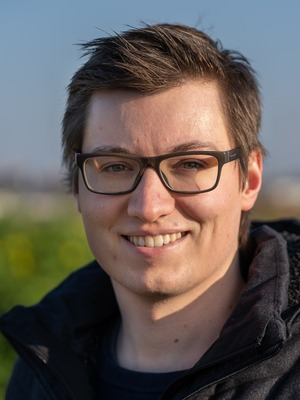
\includegraphics[height=\textwidth]{images/max.jpg}
    \end{column}%
  \end{columns}%
\end{frame}

\copywarning{}

\section[Version Control]{What is version control and why do we need it?}

\begin{frame}[c]%
  \begin{center}%
    \Huge\color{vertexDarkRed}What is version control and why do we need it?%
  \end{center}%
\end{frame}%


\begin{frame}[c]{What is Version Control?}
  \begin{itemize}
    \item Version Control tracks changes of a (collection of) document(s)
    \item This can basically be anything:
      \begin{itemize}
        \item software
        \item legal documents
        \item documentation
        \item scientific paper
        \item images
        \item ...
      \end{itemize}
    \item We will call a snapshot of such a collection a \enquote{revision}.
    \item Revisions are the complete history of our projects
  \end{itemize}
\end{frame}

\begin{frame}[c]{Why Use Version Control?}
  \begin{itemize}
    \item Allows us to go back to arbitrary revisions
    \item Shows differences between revisions
    \item Enables collaborative working
    \item Acts as backup
  \end{itemize}
\end{frame}

\begin{frame}[c]{Why Use Version Control?}
  Most Version Control Systems (VCS) make answering the following questions easy:
  \begin{description}
    \item[What?] What changed from revision \emph{A} to revision \emph{B}?
    \item[Who?] Who made a change? Who contributed?
    \item[Why?] VCS usually encourage or even force adding explanations to changes.
    \item[When?] In which revision was a bug introduced or fixed?
  \end{description}

  \onslide<2>{%
    \begin{center}
      \Large\textcolor{vertexDarkRed}{Version Control is a basic requirement for reproducible science}  
    \end{center}
  }
\end{frame}

\PassOptionsToPackage{
  unicode,
  pdfusetitle,
  colorlinks,
  linkcolor=vertexDarkRed,
  urlcolor=vertexDarkRed,
  citecolor=vertexDarkRed,
}{hyperref}
\documentclass[
  aspectratio=1610,
]{beamer}
\usetheme{vertex}
\usepackage[american]{babel}

\usepackage[autostyle]{csquotes}

\usepackage{fontspec}
\usepackage{fontawesome5}
\usepackage{graphicx}

\usepackage{tabu}

\usepackage[outputdir=build]{minted}
\usepackage{xcolor}
\usepackage{xparse}
\usepackage{tcolorbox}
\tcbuselibrary{minted}
\tcbuselibrary{skins}
\tcbuselibrary{xparse}
\usepackage{accsupp}

\usepackage{tikz}
\usetikzlibrary{
  graphs, arrows, positioning, graphdrawing
}
\usegdlibrary{trees,layered}

\usepackage{bookmark}
\usepackage[shortcuts]{extdash}


\definecolor{positive}{HTML}{15B01A}
\colorlet{negative}{vertexDarkRed}
\setmonofont{Fira Mono}

\newcommand\headline[1]{\textbf{\Large\strut{}#1}\newline}
\newcommand\headlineframe[1]{%
  \begin{frame}[c]%
    \begin{center}%
      \Huge\color{vertexDarkRed}#1%
    \end{center}%
  \end{frame}%
}%

% Codeboxes and input listings
\usemintedstyle{solarized-light}
\renewcommand\theFancyVerbLine{%
  \footnotesize%
  \textcolor{darkgray}{\arabic{FancyVerbLine}}%
}

\tcbset{basebox/.style={
  listing engine=minted,
  colback=black!5!white,
  colframe=black!60!white,
  top=0pt,
  bottom=0pt,
  left=0pt,
  right=0pt,
  enhanced,
}}

\tcbset{codeboxnumbered/.style={
  basebox,
  listing only,
  left=1em,
  overlay={%
    \begin{tcbclipinterior}
      \fill[black!20!white] (frame.south west) rectangle ([xshift=1.3em]frame.north west);
    \end{tcbclipinterior}
  },
}}


% Usage: \begin{code}[<tcolorbox options>]<minted options> {<language>} \end{code}
\DeclareTCBListing{codenumbered} {O{} D<>{} m} {
  codeboxnumbered,
  minted language=#3,
  minted options={
    fontsize=\footnotesize,
    breaklines,
    autogobble,
    linenos,
    numbersep=0.3em,
    stripnl=true,
    #2,
  },
  #1
}

\tcbset{codebox/.style={
  basebox,
  listing only,
}}


% Usage: \inputcode[<tcolorbox options>]<minted options> {<language>} {path}
\DeclareTCBInputListing{inputcode} {O{} D<>{} m m} {
  codeboxnumbered,
  listing file=#4,
  minted language=#3,
  minted options={
    fontsize=\footnotesize,
    breaklines,
    autogobble,
    stripnl=true,
    linenos,
    numbersep=0.3em,
    #2,
  },
  #1
}


% Usage: \begin{code}[<tcolorbox options>]<minted options> {<language>}\end{code}
\DeclareTCBListing{code} {O{} D<>{} m} {
  codebox,
  minted language=#3,
  minted options={
    fontsize=\footnotesize,
    breaklines,
    autogobble,
    stripnl=true,
    #2,
  },
  #1
}

\newcommand\copywarning{%
  \begin{frame}[c]{Warning}%
    \centering%
    \Large\color{vertexDarkRed}%
    \vspace{3\baselineskip}

    \begin{columns}[onlytextwidth, c]%
      \begin{column}{0.15\textwidth}%
        \fontsize{60}{60}\selectfont%
        \faIcon{biohazard}%
      \end{column}%
      \hfill%
      \begin{column}{0.7\textwidth}%
        \centering
        Copying commands or code from PDF files is\\ \textbf{dangerous}
      \end{column}%
      \hfill%
      \begin{column}{0.15\textwidth}%
        \hfill%
        \fontsize{60}{60}\selectfont%
        \hfill\faIcon{radiation}%
      \end{column}%
    \end{columns}%

    \vspace{2\baselineskip}
    Copy from the example files in the repository or type by hand.

    \bigskip
    Typing by hand is best for learning.
  \end{frame}
}


\tikzset{
  invisible/.style={opacity=0,text opacity=0},
  visible on/.style={alt={#1{}{invisible}}},
  alt/.code args={<#1>#2#3}{%
    \alt<#1>{\pgfkeysalso{#2}}{\pgfkeysalso{#3}} % \pgfkeysalso doesn't change the path
  },
}


\author[M. Nöthe]{Maximilian Nöthe}
\title[VC with Git]{Version Control using \texttt{git}}
\date[2021-06-08]{%
  \raisebox{-1.5cm}{
\includegraphics[height=3cm]{../logo-Escape_cropped.png}}
  \Large Summer School – 2022-06-21
}
\institute[TU Dortmund]{Astroparticle Physics, TU Dortmund}

\begin{document}

\maketitle

\begin{frame}[c]{Overview}
\tableofcontents
\end{frame}

\section{whoami}
\begin{frame}[c, fragile]{\texttt{whoami}}
  \begin{columns}[onlytextwidth, T]%
    \begin{column}{0.8\textwidth}%
      \begin{itemize}
        \item[{\Large\faGithub}] \href{https://github.com/maxnoe}{maxnoe}
        \item[{\Large\faUniversity}] PostDoc @ TU Dortmund
        \item[{\Large\faGraduationCap}] PhD in astroparticle physics, also @ TU Dortmund
        \item[{\Large\faFlask}] Gamma-ray astronomy with Imaging Atmospheric Cherenkov Telescopes (CTA, FACT, MAGIC)
        \item[{\Large\faMicroscope}] Data Analysis, Statistics, Machine Learning, Software Development
        \item[{\Large\faLaptopCode}] \faPython, C++, \LaTeX{}, (neo)vim, zsh, astropy, matplotlib, ...
        \item[{\Large\faHeart}] FOSS, Open Science, Best Practices
      \end{itemize}
    \end{column}%
    \hfill%
    \begin{column}{0.19\textwidth}%
      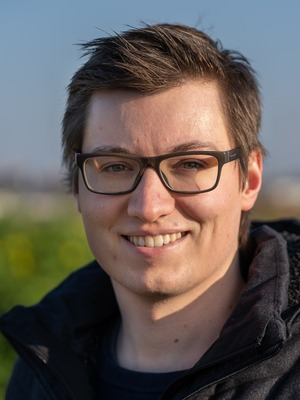
\includegraphics[height=\textwidth]{images/max.jpg}
    \end{column}%
  \end{columns}%
\end{frame}

\copywarning{}

\section[Version Control]{What is version control and why do we need it?}

\begin{frame}[c]%
  \begin{center}%
    \Huge\color{vertexDarkRed}What is version control and why do we need it?%
  \end{center}%
\end{frame}%


\begin{frame}[c]{What is Version Control?}
  \begin{itemize}
    \item Version Control tracks changes of a (collection of) document(s)
    \item This can basically be anything:
      \begin{itemize}
        \item software
        \item legal documents
        \item documentation
        \item scientific paper
        \item images
        \item ...
      \end{itemize}
    \item We will call a snapshot of such a collection a \enquote{revision}.
    \item Revisions are the complete history of our projects
  \end{itemize}
\end{frame}

\begin{frame}[c]{Why Use Version Control?}
  \begin{itemize}
    \item Allows us to go back to arbitrary revisions
    \item Shows differences between revisions
    \item Enables collaborative working
    \item Acts as backup
  \end{itemize}
\end{frame}

\begin{frame}[c]{Why Use Version Control?}
  Most Version Control Systems (VCS) make answering the following questions easy:
  \begin{description}
    \item[What?] What changed from revision \emph{A} to revision \emph{B}?
    \item[Who?] Who made a change? Who contributed?
    \item[Why?] VCS usually encourage or even force adding explanations to changes.
    \item[When?] In which revision was a bug introduced or fixed?
  \end{description}

  \onslide<2>{%
    \begin{center}
      \Large\textcolor{vertexDarkRed}{Version Control is a basic requirement for reproducible science}  
    \end{center}
  }
\end{frame}

\PassOptionsToPackage{
  unicode,
  pdfusetitle,
  colorlinks,
  linkcolor=vertexDarkRed,
  urlcolor=vertexDarkRed,
  citecolor=vertexDarkRed,
}{hyperref}
\documentclass[
  aspectratio=1610,
]{beamer}
\usetheme{vertex}
\usepackage[american]{babel}

\usepackage[autostyle]{csquotes}

\usepackage{fontspec}
\usepackage{fontawesome5}
\usepackage{graphicx}

\usepackage{tabu}

\usepackage[outputdir=build]{minted}
\usepackage{xcolor}
\usepackage{xparse}
\usepackage{tcolorbox}
\tcbuselibrary{minted}
\tcbuselibrary{skins}
\tcbuselibrary{xparse}
\usepackage{accsupp}

\usepackage{tikz}
\usetikzlibrary{
  graphs, arrows, positioning, graphdrawing
}
\usegdlibrary{trees,layered}

\usepackage{bookmark}
\usepackage[shortcuts]{extdash}


\definecolor{positive}{HTML}{15B01A}
\colorlet{negative}{vertexDarkRed}
\setmonofont{Fira Mono}

\newcommand\headline[1]{\textbf{\Large\strut{}#1}\newline}
\newcommand\headlineframe[1]{%
  \begin{frame}[c]%
    \begin{center}%
      \Huge\color{vertexDarkRed}#1%
    \end{center}%
  \end{frame}%
}%

% Codeboxes and input listings
\usemintedstyle{solarized-light}
\renewcommand\theFancyVerbLine{%
  \footnotesize%
  \textcolor{darkgray}{\arabic{FancyVerbLine}}%
}

\tcbset{basebox/.style={
  listing engine=minted,
  colback=black!5!white,
  colframe=black!60!white,
  top=0pt,
  bottom=0pt,
  left=0pt,
  right=0pt,
  enhanced,
}}

\tcbset{codeboxnumbered/.style={
  basebox,
  listing only,
  left=1em,
  overlay={%
    \begin{tcbclipinterior}
      \fill[black!20!white] (frame.south west) rectangle ([xshift=1.3em]frame.north west);
    \end{tcbclipinterior}
  },
}}


% Usage: \begin{code}[<tcolorbox options>]<minted options> {<language>} \end{code}
\DeclareTCBListing{codenumbered} {O{} D<>{} m} {
  codeboxnumbered,
  minted language=#3,
  minted options={
    fontsize=\footnotesize,
    breaklines,
    autogobble,
    linenos,
    numbersep=0.3em,
    stripnl=true,
    #2,
  },
  #1
}

\tcbset{codebox/.style={
  basebox,
  listing only,
}}


% Usage: \inputcode[<tcolorbox options>]<minted options> {<language>} {path}
\DeclareTCBInputListing{inputcode} {O{} D<>{} m m} {
  codeboxnumbered,
  listing file=#4,
  minted language=#3,
  minted options={
    fontsize=\footnotesize,
    breaklines,
    autogobble,
    stripnl=true,
    linenos,
    numbersep=0.3em,
    #2,
  },
  #1
}


% Usage: \begin{code}[<tcolorbox options>]<minted options> {<language>}\end{code}
\DeclareTCBListing{code} {O{} D<>{} m} {
  codebox,
  minted language=#3,
  minted options={
    fontsize=\footnotesize,
    breaklines,
    autogobble,
    stripnl=true,
    #2,
  },
  #1
}

\newcommand\copywarning{%
  \begin{frame}[c]{Warning}%
    \centering%
    \Large\color{vertexDarkRed}%
    \vspace{3\baselineskip}

    \begin{columns}[onlytextwidth, c]%
      \begin{column}{0.15\textwidth}%
        \fontsize{60}{60}\selectfont%
        \faIcon{biohazard}%
      \end{column}%
      \hfill%
      \begin{column}{0.7\textwidth}%
        \centering
        Copying commands or code from PDF files is\\ \textbf{dangerous}
      \end{column}%
      \hfill%
      \begin{column}{0.15\textwidth}%
        \hfill%
        \fontsize{60}{60}\selectfont%
        \hfill\faIcon{radiation}%
      \end{column}%
    \end{columns}%

    \vspace{2\baselineskip}
    Copy from the example files in the repository or type by hand.

    \bigskip
    Typing by hand is best for learning.
  \end{frame}
}


\tikzset{
  invisible/.style={opacity=0,text opacity=0},
  visible on/.style={alt={#1{}{invisible}}},
  alt/.code args={<#1>#2#3}{%
    \alt<#1>{\pgfkeysalso{#2}}{\pgfkeysalso{#3}} % \pgfkeysalso doesn't change the path
  },
}


\author[M. Nöthe]{Maximilian Nöthe}
\title[VC with Git]{Version Control using \texttt{git}}
\date[2021-06-08]{%
  \raisebox{-1.5cm}{
\includegraphics[height=3cm]{../logo-Escape_cropped.png}}
  \Large Summer School – 2022-06-21
}
\institute[TU Dortmund]{Astroparticle Physics, TU Dortmund}

\begin{document}

\maketitle

\begin{frame}[c]{Overview}
\tableofcontents
\end{frame}

\section{whoami}
\begin{frame}[c, fragile]{\texttt{whoami}}
  \begin{columns}[onlytextwidth, T]%
    \begin{column}{0.8\textwidth}%
      \begin{itemize}
        \item[{\Large\faGithub}] \href{https://github.com/maxnoe}{maxnoe}
        \item[{\Large\faUniversity}] PostDoc @ TU Dortmund
        \item[{\Large\faGraduationCap}] PhD in astroparticle physics, also @ TU Dortmund
        \item[{\Large\faFlask}] Gamma-ray astronomy with Imaging Atmospheric Cherenkov Telescopes (CTA, FACT, MAGIC)
        \item[{\Large\faMicroscope}] Data Analysis, Statistics, Machine Learning, Software Development
        \item[{\Large\faLaptopCode}] \faPython, C++, \LaTeX{}, (neo)vim, zsh, astropy, matplotlib, ...
        \item[{\Large\faHeart}] FOSS, Open Science, Best Practices
      \end{itemize}
    \end{column}%
    \hfill%
    \begin{column}{0.19\textwidth}%
      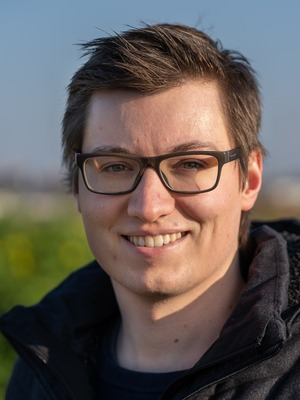
\includegraphics[height=\textwidth]{images/max.jpg}
    \end{column}%
  \end{columns}%
\end{frame}

\copywarning{}

\section[Version Control]{What is version control and why do we need it?}

\begin{frame}[c]%
  \begin{center}%
    \Huge\color{vertexDarkRed}What is version control and why do we need it?%
  \end{center}%
\end{frame}%


\begin{frame}[c]{What is Version Control?}
  \begin{itemize}
    \item Version Control tracks changes of a (collection of) document(s)
    \item This can basically be anything:
      \begin{itemize}
        \item software
        \item legal documents
        \item documentation
        \item scientific paper
        \item images
        \item ...
      \end{itemize}
    \item We will call a snapshot of such a collection a \enquote{revision}.
    \item Revisions are the complete history of our projects
  \end{itemize}
\end{frame}

\begin{frame}[c]{Why Use Version Control?}
  \begin{itemize}
    \item Allows us to go back to arbitrary revisions
    \item Shows differences between revisions
    \item Enables collaborative working
    \item Acts as backup
  \end{itemize}
\end{frame}

\begin{frame}[c]{Why Use Version Control?}
  Most Version Control Systems (VCS) make answering the following questions easy:
  \begin{description}
    \item[What?] What changed from revision \emph{A} to revision \emph{B}?
    \item[Who?] Who made a change? Who contributed?
    \item[Why?] VCS usually encourage or even force adding explanations to changes.
    \item[When?] In which revision was a bug introduced or fixed?
  \end{description}

  \onslide<2>{%
    \begin{center}
      \Large\textcolor{vertexDarkRed}{Version Control is a basic requirement for reproducible science}  
    \end{center}
  }
\end{frame}

\input{header_maxnoe.tex}

\tikzset{
  invisible/.style={opacity=0,text opacity=0},
  visible on/.style={alt={#1{}{invisible}}},
  alt/.code args={<#1>#2#3}{%
    \alt<#1>{\pgfkeysalso{#2}}{\pgfkeysalso{#3}} % \pgfkeysalso doesn't change the path
  },
}


\author[M. Nöthe]{Maximilian Nöthe}
\title[VC with Git]{Version Control using \texttt{git}}
\date[2021-06-08]{%
  \raisebox{-1.5cm}{
\includegraphics[height=3cm]{../logo-Escape_cropped.png}}
  \Large Summer School – 2022-06-21
}
\institute[TU Dortmund]{Astroparticle Physics, TU Dortmund}

\begin{document}

\maketitle

\begin{frame}[c]{Overview}
\tableofcontents
\end{frame}

\section{whoami}
\begin{frame}[c, fragile]{\texttt{whoami}}
  \begin{columns}[onlytextwidth, T]%
    \begin{column}{0.8\textwidth}%
      \begin{itemize}
        \item[{\Large\faGithub}] \href{https://github.com/maxnoe}{maxnoe}
        \item[{\Large\faUniversity}] PostDoc @ TU Dortmund
        \item[{\Large\faGraduationCap}] PhD in astroparticle physics, also @ TU Dortmund
        \item[{\Large\faFlask}] Gamma-ray astronomy with Imaging Atmospheric Cherenkov Telescopes (CTA, FACT, MAGIC)
        \item[{\Large\faMicroscope}] Data Analysis, Statistics, Machine Learning, Software Development
        \item[{\Large\faLaptopCode}] \faPython, C++, \LaTeX{}, (neo)vim, zsh, astropy, matplotlib, ...
        \item[{\Large\faHeart}] FOSS, Open Science, Best Practices
      \end{itemize}
    \end{column}%
    \hfill%
    \begin{column}{0.19\textwidth}%
      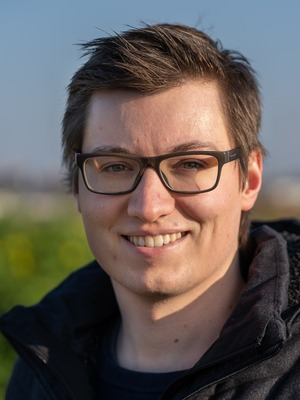
\includegraphics[height=\textwidth]{images/max.jpg}
    \end{column}%
  \end{columns}%
\end{frame}

\copywarning{}

\input{content/vc.tex}
\input{content/git.tex}
\headlineframe{Questions?}

\input{content/hosters.tex}
\input{content/advanced.tex}
\headlineframe{Questions?}

\end{document}

\headlineframe{Questions?}

\section{Git Hosting Providers}
\headlineframe{Git Hosting Providers}

\begin{frame}[c]{Git Hosting Providers}
  \begin{itemize}
    \item Several Providers and self-hosted server solutions are available
    \item Usually provide much more than just hosting the repositories
      \begin{itemize}
        \item Issue tracking
        \item Code review using pull requests
        \item Wiki
        \item Project Management, e.g. Canban boards
        \item Continuous integration
        \item Releases
      \end{itemize}
  \end{itemize}
\end{frame}

\begin{frame}[c]{Git Hosting Providers}
  \small
  \begin{tabu}{@{} X[,C] @{} X[,C] @{} X[,C] @{}}
    \href{https://github.com}{\includegraphics[width=0.75\linewidth]{figures/github.png}} &
    \href{https://gitlab.com}{\includegraphics[width=0.75\linewidth]{figures/gitlab.png}} &
    \href{https://bitbucket.org}{\includegraphics[width=0.75\linewidth]{figures/bitbucket.png}} \\
    \begin{itemize}
      \item Largest Hoster
      \item Many Open Source Projects, e.g. Python
      \item Unlimited private repositories
      \item Free CI service for public repositories
      \item Github Pro free for students / teachers / researchers
    \end{itemize}
    &
    \begin{itemize}
      \item open-source community edition
      \item paid enterprise edition with more features
      \item unlimited private repositories
      \item Self hosted or as service at \href{https://gitlab.com}{gitlab.com}
    \end{itemize}
    &
    \begin{itemize}
      \item Unlimited private repos with up to 5 contributors
      \item Lacks far behind GitHub and GitLab
    \end{itemize}
  \end{tabu}
\end{frame}

\begin{frame}[fragile]{SSH Keys}
  Git can communicate using two ways with a remote:
  \begin{description}
    \item[HTTPS] Works out of the box but requires entering credentials at every push/pull
    \item[SSH] Using private/public keys. \\ Usually, you only need to decrypt a key once per session.
  \end{description}

  \begin{itemize}
    \item To use ssh, you need to add at least one public key to your profile. 
    \item It is considered best practice to use unique keys per machine and service
  \end{itemize}

  \begin{enumerate}
    \item Create the key using: (choose a new password when asked)
      \begin{code}[title={Works in Powershell (Windows) and Unix Systems}]{bash}
        $ ssh-keygen -t ed25519 -C "GitHub Key for <username> at <machine>" -f "$HOME/.ssh/id_ed25519.github"
      \end{code}
    \item Copy the content of the public key, on unix with \mintinline{bash}+cat ~/.ssh/id_rsa.github.pub+ or by using a text editor to open the file
    \item Add the public key to your profile
  \end{enumerate}
\end{frame}

\begin{frame}[c]{Pull / Merge Requests}
  \begin{itemize}
    \item Pull Requests (GitHub) / Merge Requests (GitLab) are a feature on top of git provided by several platforms
    \item Used to propose changes by pushing a new branch and then requesting it to be merged into the main branch
    \item Usually, projects using the GitHub Workflow only allow changes to the master branch via Pull Requests
    \item Pull Requests are used for Code Review, project maintainers and co-developers can look at your code and
      ask for changes
    \item Usually, a Continuous Integration (CI) system runs checks for the changes proposed in a Pull Request
  \end{itemize}
\end{frame}

\begin{frame}[c]{Code Reviews}
  \begin{itemize}
    \item Code reviews are among the most essential parts of software development
    \item Similar to the peer-review process in science
    \item Get feedback and advice for improvements
    \item Prevent easy-to-find mistakes
    \item Ensure quality, performance, documentation, clarity of the software
    \item Developers can learn from each other immensely during code reviews
    \item You should require code reviews for pull requests
  \end{itemize}
\end{frame}

\begin{frame}[c]{How should you review code?}
  \begin{itemize}
    \item Automatize as much as possible before the actual human review
      \begin{itemize}
        \item Static code checks
        \item Unit tests / CI
        \item Coverage
        \item Code style checks
      \end{itemize}
    \item Focus on (in order):
      \begin{itemize}
        \item[\color{positive}\faCheckSquare] Are enough unit tests there?
        \item[\color{positive}\faCheckSquare] Are code and tests clear / explained in comments / following best practices?
        \item[\color{positive}\faCheckSquare] Any obvious performance improvements?\footnote{\enquote{Premature optimization is the root of all evil} –  Donald Knuth}
        \item[\color{positive}\faCheckSquare] Is the code documented?
      \end{itemize}
    \item Stay friendly but be concise
  \end{itemize}
\end{frame}


\begin{frame}[c]{Forking}
  \begin{itemize}
    \item Using git and hosting providers, it's easy to contribute to projects you do not have write access to.

    \item This is arguably the most important reason for git's success.

    \item Forking means to create a copy of the main repository in your namespace, e.g. \url{http://github.com/matplotlib/matplotlib} to \texttt{http://github.com/maxnoe/matplotlib}

    \item You can then make changes and create a pull request in the main repository!

    \item To keep your fork up to date, you should add both your fork and the main repo as remotes.
  \end{itemize}
\end{frame}

\begin{frame}[fragile]{Forks}
  We'll use the school repository for this example

  \begin{itemize}
    \item Click the \enquote{Fork} button on GitHub
    \item Clone your fork
      \begin{code}{bash}
        $ git clone git@github.com:maxnoe/school2021
      \end{code}
    \item Add the main repository as second remote. The name \enquote{upstream} is convention.
      \begin{code}{bash}
        $ git remote add upstream git@github.com:escape2020/school2021
      \end{code}
    \item Download content also from upstream
      \begin{code}{bash}
        $ git fetch upstream
      \end{code}
  \end{itemize}
\end{frame}

\begin{frame}[c, fragile]{Making a Pull Request from a forked Repository}
  \begin{itemize}
    \item When starting the new branch, make sure to start from the up-to-date upstream main/master:
      \begin{code}{bash}
        $ git fetch upstream
        $ git switch -c new_branch upstream/master
      \end{code}
    \item Make changes and commit
    \item When pushing the branch, specify your fork (origin):
      \begin{code}{bash}
        $ git push -u origin new_branch
      \end{code}
    \item Go to GitHub or click on the link in the push message to open the Pull Request
  \end{itemize}
\end{frame}

\begin{frame}[c]{Issue Tracking}
  \begin{itemize}
    \item Issue Trackers are an important part of every software project
      \begin{itemize}
        \item Report bugs
        \item Feature requests
        \item Project planning
        \item Ask for help
      \end{itemize}
    \item Issues can be linked to commits and pull requests
  \end{itemize}
\end{frame}

\begin{frame}[c, fragile]{Commit Integration with Issue Tracking}
  Start working on fixing a bug, that was documented in issue 42.

  \begin{code}{text}
  $ git checkout -b fix_42

  ... do stuff to fix bug ...

  $ git add src/foo.cxx
  $ git commit -m "Fix segmentation fault when doing stuff, fixes #42" 
  $ git push -u origin fix_42
  \end{code}

  If this commit get's merged into master, issue 42 will automatically be closed.
\end{frame}

\begin{frame}[c]{Continuous Integration}
  \begin{itemize}
    \item Strictly interpreted, continous integration means integrating current work
      \enquote{often} into the main version
    \item Usually, this means running automated builds and checks on a dedicated server
    \item Ideally, these are run for each push event
    \item For git projects, checks for pull requests should run on the merged result, not the branch itself
    \item You should require passing CI system for Pull Requests
  \end{itemize}
\end{frame}

\begin{frame}[c]{Common Features of CI systems}
  \begin{itemize}
    \item Build your application / library
    \item Run the test suite
    \item Do that for multiple OSes and software / compiler versions
    \item Build documentation and packages
    \item Upload and publish results / build products
  \end{itemize}
\end{frame}

\begin{frame}[c, fragile]{Example python workflow}
  \begin{center}\large
    \url{https://github.com/maxnoe/pyfibonacci/blob/main/.github/workflows/ci.yml}

    More details during the testing lecture.
  \end{center}
\end{frame}

\section{Advanced Git}
\headlineframe{Advanced Git}

\begin{frame}[c, fragile]{Partial Adding}
  \begin{itemize}
    \item Commits should be small, logically contained units
    \item Sometimes, we implement multiple things in one go 
    \item Go through all changes interactively, select what we want to add with
      \begin{code}{bash}
        $ git add -p
      \end{code}
  \end{itemize}
\end{frame}

\headlineframe{%
  Changing the git history\\
  (aka the danger zone)
}%

\begin{frame}[c]{Disclaimers}
  \begin{itemize}
    \item The main/main branch's history should only be modified under severe circumstances\\
      \begin{itemize}
        \item Sensitive data in the history\footnote{Under most circumstances I wouldn't recomend to change the history. Change the passwords.}
        \item Large files in the history that need to be removed
      \end{itemize}
    \item Not-yet-pushed commits can be freely modified
    \item Feature branches can usually be modified
    \item Most large projects will even ask you to cleanup the history of your Pull Request to have a \enquote{nice} history
    \item Modifying already-pushed commits requires pushing with the \mintinline{bash}+--force+ option
    \item The main/main branch should be protected against force pushes\\
      (Github/Gitlab settings)
  \end{itemize}
\end{frame}

\begin{frame}[c, fragile]{Fixing the last commit}
  \begin{itemize}
    \item Just changing the last commit is one of the most common use cases
      \begin{itemize}
        \item Fix a typo in the commit message
        \item Add a forgotten file
        \item Remove an accidentally commit file
      \end{itemize}
    \item Make and add the changes you want to include / fix in the last commit
    \item Execute
      \begin{code}{bash}
        $ git commit --amend
      \end{code}
      \begin{itemize}
        \item Adds the current staging area to the last commit (optional)
        \item Opens the editor for editing the commit message
        \item Overwrites the last commit (will change the hash)
      \end{itemize}
  \end{itemize}
\end{frame}

\begin{frame}[c]{Rebase - rewriting the git history}
  Rebase is a very powerful tool to rewrite the git history.

  It can
  \begin{itemize}
    \item Change commit order
    \item Drop / edit single commits
    \item Merge multiple commits into one
  \end{itemize}
\end{frame}


\begin{frame}[t, fragile]{Merge vs.\ Rebase}
  \begin{itemize}
    \item Default behaviour of \mintinline{bash}+git pull+ is equivalent to \mintinline{bash}+git fetch && git merge <remote>/<branch>+
    \item This results in a non-linear history with many merge conflicts like \enquote{Merging remote tracking branch...}
    \item \mintinline{bash}+git pull --rebase+ is equivalent to \mintinline{bash}+git fetch && git rebase <remote>/<branch>+
    \item It makes the history equal to the remote history, and then tries to apply the local commits in order
  \end{itemize}

  Can be made the default with \mintinline{bash}+git config --global pull.rebase true+

  Changes how conflicts are resolved: Instead of creating a single merge commit that 
  contains the fixes to make the two parents compatible, each commit that is rebased is adapted
  so the conflicts never existed.
\end{frame}

\begin{frame}[t, fragile]{\mintinline{bash}+git pull --rebase+ vs.\ \mintinline{bash}+git pull --merge+}
  \begin{columns}[onlytextwidth, t]
    \begin{column}{0.22\textwidth}
      Situation at start

      \begin{tikzpicture}
        \graph [
          layered layout,
          nodes={
            blue!70!black,
            node font=\ttfamily,
          },
        ]{
          a <- b <- c <- d <- e <- main [vertexDarkRed];
          b <- 1 <- 2 <- you [vertexDarkRed];
        };
      \end{tikzpicture}
    \end{column}
    \hfill
    \begin{column}{0.22\textwidth}
      With merging

      \begin{tikzpicture}
        \graph [
          layered layout,
          nodes={
            blue!70!black,
            node font=\ttfamily,
          },
        ]{
          a <- b <- c <- d <- e <- f;
          b <- 1 <- 2 <- 3;
          d <- 3;
          3 <- f;
          f <- main [vertexDarkRed];
        };
      \end{tikzpicture}
    \end{column}
    \hfill
    \begin{column}{0.22\textwidth}
      After rebase

      \begin{tikzpicture}
        \graph [
          layered layout,
          nodes={
            blue!70!black,
            node font=\ttfamily,
          },
        ]{
          a <- b <- c <- d <- e <-  main [vertexDarkRed];
          e <- 1 <- 2 <- you [vertexDarkRed];
        };
      \end{tikzpicture}
    \end{column}
    \hfill
    \begin{column}{0.22\textwidth}
      After merging the rebased branch

      \begin{tikzpicture}
        \graph [
          layered layout,
          nodes={
            blue!70!black,
            node font=\ttfamily,
          },
        ]{
          c <- d <- e <- f <- main [vertexDarkRed];
          e <- 1 <- 2;
          2 <- f;
        };
      \end{tikzpicture}
    \end{column}
  \end{columns}
\end{frame}


\begin{frame}[c, fragile]{Interactive Rebase}
  \begin{itemize}
    \item Very powerful tool to change commits 
    \item Joining / dropping / reordering / changing commits
  \end{itemize}
  \begin{code}{bash}
    $ git rebase -i <target commit>
  \end{code}
\end{frame}

\begin{frame}[c, fragile]{Submodules}
  \begin{itemize}
    \item Git discourages mono-repositories with many projects or
      just adding other projects to a repository
    \item Useful for 
      \begin{itemize}
        \item external source dependencies (e.\,g.\ Google Test for C++ projects)
        \item meta-repositories joining multiple repositores at specific versions
      \end{itemize}
    \item Submodules add a reference to another repository at a certain commit:
      \begin{code}{bash}
        $ git submodule add <url> <path>
      \end{code}
    \item Cloning does not include submodules by default, needs
      \begin{code}{bash}
        $ git clone <url> --recursive
      \end{code}
    \item Update submodules (e.\,g.\ if changed on the remote)
      \begin{code}{bash}
        $ git submodule update --init --recursive
      \end{code}
  \end{itemize}
\end{frame}

\headlineframe{Questions?}

\end{document}

\headlineframe{Questions?}

\section{Git Hosting Providers}
\headlineframe{Git Hosting Providers}

\begin{frame}[c]{Git Hosting Providers}
  \begin{itemize}
    \item Several Providers and self-hosted server solutions are available
    \item Usually provide much more than just hosting the repositories
      \begin{itemize}
        \item Issue tracking
        \item Code review using pull requests
        \item Wiki
        \item Project Management, e.g. Canban boards
        \item Continuous integration
        \item Releases
      \end{itemize}
  \end{itemize}
\end{frame}

\begin{frame}[c]{Git Hosting Providers}
  \small
  \begin{tabu}{@{} X[,C] @{} X[,C] @{} X[,C] @{}}
    \href{https://github.com}{\includegraphics[width=0.75\linewidth]{figures/github.png}} &
    \href{https://gitlab.com}{\includegraphics[width=0.75\linewidth]{figures/gitlab.png}} &
    \href{https://bitbucket.org}{\includegraphics[width=0.75\linewidth]{figures/bitbucket.png}} \\
    \begin{itemize}
      \item Largest Hoster
      \item Many Open Source Projects, e.g. Python
      \item Unlimited private repositories
      \item Free CI service for public repositories
      \item Github Pro free for students / teachers / researchers
    \end{itemize}
    &
    \begin{itemize}
      \item open-source community edition
      \item paid enterprise edition with more features
      \item unlimited private repositories
      \item Self hosted or as service at \href{https://gitlab.com}{gitlab.com}
    \end{itemize}
    &
    \begin{itemize}
      \item Unlimited private repos with up to 5 contributors
      \item Lacks far behind GitHub and GitLab
    \end{itemize}
  \end{tabu}
\end{frame}

\begin{frame}[fragile]{SSH Keys}
  Git can communicate using two ways with a remote:
  \begin{description}
    \item[HTTPS] Works out of the box but requires entering credentials at every push/pull
    \item[SSH] Using private/public keys. \\ Usually, you only need to decrypt a key once per session.
  \end{description}

  \begin{itemize}
    \item To use ssh, you need to add at least one public key to your profile. 
    \item It is considered best practice to use unique keys per machine and service
  \end{itemize}

  \begin{enumerate}
    \item Create the key using: (choose a new password when asked)
      \begin{code}[title={Works in Powershell (Windows) and Unix Systems}]{bash}
        $ ssh-keygen -t ed25519 -C "GitHub Key for <username> at <machine>" -f "$HOME/.ssh/id_ed25519.github"
      \end{code}
    \item Copy the content of the public key, on unix with \mintinline{bash}+cat ~/.ssh/id_rsa.github.pub+ or by using a text editor to open the file
    \item Add the public key to your profile
  \end{enumerate}
\end{frame}

\begin{frame}[c]{Pull / Merge Requests}
  \begin{itemize}
    \item Pull Requests (GitHub) / Merge Requests (GitLab) are a feature on top of git provided by several platforms
    \item Used to propose changes by pushing a new branch and then requesting it to be merged into the main branch
    \item Usually, projects using the GitHub Workflow only allow changes to the master branch via Pull Requests
    \item Pull Requests are used for Code Review, project maintainers and co-developers can look at your code and
      ask for changes
    \item Usually, a Continuous Integration (CI) system runs checks for the changes proposed in a Pull Request
  \end{itemize}
\end{frame}

\begin{frame}[c]{Code Reviews}
  \begin{itemize}
    \item Code reviews are among the most essential parts of software development
    \item Similar to the peer-review process in science
    \item Get feedback and advice for improvements
    \item Prevent easy-to-find mistakes
    \item Ensure quality, performance, documentation, clarity of the software
    \item Developers can learn from each other immensely during code reviews
    \item You should require code reviews for pull requests
  \end{itemize}
\end{frame}

\begin{frame}[c]{How should you review code?}
  \begin{itemize}
    \item Automatize as much as possible before the actual human review
      \begin{itemize}
        \item Static code checks
        \item Unit tests / CI
        \item Coverage
        \item Code style checks
      \end{itemize}
    \item Focus on (in order):
      \begin{itemize}
        \item[\color{positive}\faCheckSquare] Are enough unit tests there?
        \item[\color{positive}\faCheckSquare] Are code and tests clear / explained in comments / following best practices?
        \item[\color{positive}\faCheckSquare] Any obvious performance improvements?\footnote{\enquote{Premature optimization is the root of all evil} –  Donald Knuth}
        \item[\color{positive}\faCheckSquare] Is the code documented?
      \end{itemize}
    \item Stay friendly but be concise
  \end{itemize}
\end{frame}


\begin{frame}[c]{Forking}
  \begin{itemize}
    \item Using git and hosting providers, it's easy to contribute to projects you do not have write access to.

    \item This is arguably the most important reason for git's success.

    \item Forking means to create a copy of the main repository in your namespace, e.g. \url{http://github.com/matplotlib/matplotlib} to \texttt{http://github.com/maxnoe/matplotlib}

    \item You can then make changes and create a pull request in the main repository!

    \item To keep your fork up to date, you should add both your fork and the main repo as remotes.
  \end{itemize}
\end{frame}

\begin{frame}[fragile]{Forks}
  We'll use the school repository for this example

  \begin{itemize}
    \item Click the \enquote{Fork} button on GitHub
    \item Clone your fork
      \begin{code}{bash}
        $ git clone git@github.com:maxnoe/school2021
      \end{code}
    \item Add the main repository as second remote. The name \enquote{upstream} is convention.
      \begin{code}{bash}
        $ git remote add upstream git@github.com:escape2020/school2021
      \end{code}
    \item Download content also from upstream
      \begin{code}{bash}
        $ git fetch upstream
      \end{code}
  \end{itemize}
\end{frame}

\begin{frame}[c, fragile]{Making a Pull Request from a forked Repository}
  \begin{itemize}
    \item When starting the new branch, make sure to start from the up-to-date upstream main/master:
      \begin{code}{bash}
        $ git fetch upstream
        $ git switch -c new_branch upstream/master
      \end{code}
    \item Make changes and commit
    \item When pushing the branch, specify your fork (origin):
      \begin{code}{bash}
        $ git push -u origin new_branch
      \end{code}
    \item Go to GitHub or click on the link in the push message to open the Pull Request
  \end{itemize}
\end{frame}

\begin{frame}[c]{Issue Tracking}
  \begin{itemize}
    \item Issue Trackers are an important part of every software project
      \begin{itemize}
        \item Report bugs
        \item Feature requests
        \item Project planning
        \item Ask for help
      \end{itemize}
    \item Issues can be linked to commits and pull requests
  \end{itemize}
\end{frame}

\begin{frame}[c, fragile]{Commit Integration with Issue Tracking}
  Start working on fixing a bug, that was documented in issue 42.

  \begin{code}{text}
  $ git checkout -b fix_42

  ... do stuff to fix bug ...

  $ git add src/foo.cxx
  $ git commit -m "Fix segmentation fault when doing stuff, fixes #42" 
  $ git push -u origin fix_42
  \end{code}

  If this commit get's merged into master, issue 42 will automatically be closed.
\end{frame}

\begin{frame}[c]{Continuous Integration}
  \begin{itemize}
    \item Strictly interpreted, continous integration means integrating current work
      \enquote{often} into the main version
    \item Usually, this means running automated builds and checks on a dedicated server
    \item Ideally, these are run for each push event
    \item For git projects, checks for pull requests should run on the merged result, not the branch itself
    \item You should require passing CI system for Pull Requests
  \end{itemize}
\end{frame}

\begin{frame}[c]{Common Features of CI systems}
  \begin{itemize}
    \item Build your application / library
    \item Run the test suite
    \item Do that for multiple OSes and software / compiler versions
    \item Build documentation and packages
    \item Upload and publish results / build products
  \end{itemize}
\end{frame}

\begin{frame}[c, fragile]{Example python workflow}
  \begin{center}\large
    \url{https://github.com/maxnoe/pyfibonacci/blob/main/.github/workflows/ci.yml}

    More details during the testing lecture.
  \end{center}
\end{frame}

\section{Advanced Git}
\headlineframe{Advanced Git}

\begin{frame}[c, fragile]{Partial Adding}
  \begin{itemize}
    \item Commits should be small, logically contained units
    \item Sometimes, we implement multiple things in one go 
    \item Go through all changes interactively, select what we want to add with
      \begin{code}{bash}
        $ git add -p
      \end{code}
  \end{itemize}
\end{frame}

\headlineframe{%
  Changing the git history\\
  (aka the danger zone)
}%

\begin{frame}[c]{Disclaimers}
  \begin{itemize}
    \item The main/main branch's history should only be modified under severe circumstances\\
      \begin{itemize}
        \item Sensitive data in the history\footnote{Under most circumstances I wouldn't recomend to change the history. Change the passwords.}
        \item Large files in the history that need to be removed
      \end{itemize}
    \item Not-yet-pushed commits can be freely modified
    \item Feature branches can usually be modified
    \item Most large projects will even ask you to cleanup the history of your Pull Request to have a \enquote{nice} history
    \item Modifying already-pushed commits requires pushing with the \mintinline{bash}+--force+ option
    \item The main/main branch should be protected against force pushes\\
      (Github/Gitlab settings)
  \end{itemize}
\end{frame}

\begin{frame}[c, fragile]{Fixing the last commit}
  \begin{itemize}
    \item Just changing the last commit is one of the most common use cases
      \begin{itemize}
        \item Fix a typo in the commit message
        \item Add a forgotten file
        \item Remove an accidentally commit file
      \end{itemize}
    \item Make and add the changes you want to include / fix in the last commit
    \item Execute
      \begin{code}{bash}
        $ git commit --amend
      \end{code}
      \begin{itemize}
        \item Adds the current staging area to the last commit (optional)
        \item Opens the editor for editing the commit message
        \item Overwrites the last commit (will change the hash)
      \end{itemize}
  \end{itemize}
\end{frame}

\begin{frame}[c]{Rebase - rewriting the git history}
  Rebase is a very powerful tool to rewrite the git history.

  It can
  \begin{itemize}
    \item Change commit order
    \item Drop / edit single commits
    \item Merge multiple commits into one
  \end{itemize}
\end{frame}


\begin{frame}[t, fragile]{Merge vs.\ Rebase}
  \begin{itemize}
    \item Default behaviour of \mintinline{bash}+git pull+ is equivalent to \mintinline{bash}+git fetch && git merge <remote>/<branch>+
    \item This results in a non-linear history with many merge conflicts like \enquote{Merging remote tracking branch...}
    \item \mintinline{bash}+git pull --rebase+ is equivalent to \mintinline{bash}+git fetch && git rebase <remote>/<branch>+
    \item It makes the history equal to the remote history, and then tries to apply the local commits in order
  \end{itemize}

  Can be made the default with \mintinline{bash}+git config --global pull.rebase true+

  Changes how conflicts are resolved: Instead of creating a single merge commit that 
  contains the fixes to make the two parents compatible, each commit that is rebased is adapted
  so the conflicts never existed.
\end{frame}

\begin{frame}[t, fragile]{\mintinline{bash}+git pull --rebase+ vs.\ \mintinline{bash}+git pull --merge+}
  \begin{columns}[onlytextwidth, t]
    \begin{column}{0.22\textwidth}
      Situation at start

      \begin{tikzpicture}
        \graph [
          layered layout,
          nodes={
            blue!70!black,
            node font=\ttfamily,
          },
        ]{
          a <- b <- c <- d <- e <- main [vertexDarkRed];
          b <- 1 <- 2 <- you [vertexDarkRed];
        };
      \end{tikzpicture}
    \end{column}
    \hfill
    \begin{column}{0.22\textwidth}
      With merging

      \begin{tikzpicture}
        \graph [
          layered layout,
          nodes={
            blue!70!black,
            node font=\ttfamily,
          },
        ]{
          a <- b <- c <- d <- e <- f;
          b <- 1 <- 2 <- 3;
          d <- 3;
          3 <- f;
          f <- main [vertexDarkRed];
        };
      \end{tikzpicture}
    \end{column}
    \hfill
    \begin{column}{0.22\textwidth}
      After rebase

      \begin{tikzpicture}
        \graph [
          layered layout,
          nodes={
            blue!70!black,
            node font=\ttfamily,
          },
        ]{
          a <- b <- c <- d <- e <-  main [vertexDarkRed];
          e <- 1 <- 2 <- you [vertexDarkRed];
        };
      \end{tikzpicture}
    \end{column}
    \hfill
    \begin{column}{0.22\textwidth}
      After merging the rebased branch

      \begin{tikzpicture}
        \graph [
          layered layout,
          nodes={
            blue!70!black,
            node font=\ttfamily,
          },
        ]{
          c <- d <- e <- f <- main [vertexDarkRed];
          e <- 1 <- 2;
          2 <- f;
        };
      \end{tikzpicture}
    \end{column}
  \end{columns}
\end{frame}


\begin{frame}[c, fragile]{Interactive Rebase}
  \begin{itemize}
    \item Very powerful tool to change commits 
    \item Joining / dropping / reordering / changing commits
  \end{itemize}
  \begin{code}{bash}
    $ git rebase -i <target commit>
  \end{code}
\end{frame}

\begin{frame}[c, fragile]{Submodules}
  \begin{itemize}
    \item Git discourages mono-repositories with many projects or
      just adding other projects to a repository
    \item Useful for 
      \begin{itemize}
        \item external source dependencies (e.\,g.\ Google Test for C++ projects)
        \item meta-repositories joining multiple repositores at specific versions
      \end{itemize}
    \item Submodules add a reference to another repository at a certain commit:
      \begin{code}{bash}
        $ git submodule add <url> <path>
      \end{code}
    \item Cloning does not include submodules by default, needs
      \begin{code}{bash}
        $ git clone <url> --recursive
      \end{code}
    \item Update submodules (e.\,g.\ if changed on the remote)
      \begin{code}{bash}
        $ git submodule update --init --recursive
      \end{code}
  \end{itemize}
\end{frame}

\headlineframe{Questions?}

\end{document}

\headlineframe{Questions?}

\section{Git Hosting Providers}
\headlineframe{Git Hosting Providers}

\begin{frame}[c]{Git Hosting Providers}
  \begin{itemize}
    \item Several Providers and self-hosted server solutions are available
    \item Usually provide much more than just hosting the repositories
      \begin{itemize}
        \item Issue tracking
        \item Code review using pull requests
        \item Wiki
        \item Project Management, e.g. Canban boards
        \item Continuous integration
        \item Releases
      \end{itemize}
  \end{itemize}
\end{frame}

\begin{frame}[c]{Git Hosting Providers}
  \small
  \begin{tabu}{@{} X[,C] @{} X[,C] @{} X[,C] @{}}
    \href{https://github.com}{\includegraphics[width=0.75\linewidth]{figures/github.png}} &
    \href{https://gitlab.com}{\includegraphics[width=0.75\linewidth]{figures/gitlab.png}} &
    \href{https://bitbucket.org}{\includegraphics[width=0.75\linewidth]{figures/bitbucket.png}} \\
    \begin{itemize}
      \item Largest Hoster
      \item Many Open Source Projects, e.g. Python
      \item Unlimited private repositories
      \item Free CI service for public repositories
      \item Github Pro free for students / teachers / researchers
    \end{itemize}
    &
    \begin{itemize}
      \item open-source community edition
      \item paid enterprise edition with more features
      \item unlimited private repositories
      \item Self hosted or as service at \href{https://gitlab.com}{gitlab.com}
    \end{itemize}
    &
    \begin{itemize}
      \item Unlimited private repos with up to 5 contributors
      \item Lacks far behind GitHub and GitLab
    \end{itemize}
  \end{tabu}
\end{frame}

\begin{frame}[fragile]{SSH Keys}
  Git can communicate using two ways with a remote:
  \begin{description}
    \item[HTTPS] Works out of the box but requires entering credentials at every push/pull
    \item[SSH] Using private/public keys. \\ Usually, you only need to decrypt a key once per session.
  \end{description}

  \begin{itemize}
    \item To use ssh, you need to add at least one public key to your profile. 
    \item It is considered best practice to use unique keys per machine and service
  \end{itemize}

  \begin{enumerate}
    \item Create the key using: (choose a new password when asked)
      \begin{code}[title={Works in Powershell (Windows) and Unix Systems}]{bash}
        $ ssh-keygen -t ed25519 -C "GitHub Key for <username> at <machine>" -f "$HOME/.ssh/id_ed25519.github"
      \end{code}
    \item Copy the content of the public key, on unix with \mintinline{bash}+cat ~/.ssh/id_rsa.github.pub+ or by using a text editor to open the file
    \item Add the public key to your profile
  \end{enumerate}
\end{frame}

\begin{frame}[c]{Pull / Merge Requests}
  \begin{itemize}
    \item Pull Requests (GitHub) / Merge Requests (GitLab) are a feature on top of git provided by several platforms
    \item Used to propose changes by pushing a new branch and then requesting it to be merged into the main branch
    \item Usually, projects using the GitHub Workflow only allow changes to the master branch via Pull Requests
    \item Pull Requests are used for Code Review, project maintainers and co-developers can look at your code and
      ask for changes
    \item Usually, a Continuous Integration (CI) system runs checks for the changes proposed in a Pull Request
  \end{itemize}
\end{frame}

\begin{frame}[c]{Code Reviews}
  \begin{itemize}
    \item Code reviews are among the most essential parts of software development
    \item Similar to the peer-review process in science
    \item Get feedback and advice for improvements
    \item Prevent easy-to-find mistakes
    \item Ensure quality, performance, documentation, clarity of the software
    \item Developers can learn from each other immensely during code reviews
    \item You should require code reviews for pull requests
  \end{itemize}
\end{frame}

\begin{frame}[c]{How should you review code?}
  \begin{itemize}
    \item Automatize as much as possible before the actual human review
      \begin{itemize}
        \item Static code checks
        \item Unit tests / CI
        \item Coverage
        \item Code style checks
      \end{itemize}
    \item Focus on (in order):
      \begin{itemize}
        \item[\color{positive}\faCheckSquare] Are enough unit tests there?
        \item[\color{positive}\faCheckSquare] Are code and tests clear / explained in comments / following best practices?
        \item[\color{positive}\faCheckSquare] Any obvious performance improvements?\footnote{\enquote{Premature optimization is the root of all evil} –  Donald Knuth}
        \item[\color{positive}\faCheckSquare] Is the code documented?
      \end{itemize}
    \item Stay friendly but be concise
  \end{itemize}
\end{frame}


\begin{frame}[c]{Forking}
  \begin{itemize}
    \item Using git and hosting providers, it's easy to contribute to projects you do not have write access to.

    \item This is arguably the most important reason for git's success.

    \item Forking means to create a copy of the main repository in your namespace, e.g. \url{http://github.com/matplotlib/matplotlib} to \texttt{http://github.com/maxnoe/matplotlib}

    \item You can then make changes and create a pull request in the main repository!

    \item To keep your fork up to date, you should add both your fork and the main repo as remotes.
  \end{itemize}
\end{frame}

\begin{frame}[fragile]{Forks}
  We'll use the school repository for this example

  \begin{itemize}
    \item Click the \enquote{Fork} button on GitHub
    \item Clone your fork
      \begin{code}{bash}
        $ git clone git@github.com:maxnoe/school2021
      \end{code}
    \item Add the main repository as second remote. The name \enquote{upstream} is convention.
      \begin{code}{bash}
        $ git remote add upstream git@github.com:escape2020/school2021
      \end{code}
    \item Download content also from upstream
      \begin{code}{bash}
        $ git fetch upstream
      \end{code}
  \end{itemize}
\end{frame}

\begin{frame}[c, fragile]{Making a Pull Request from a forked Repository}
  \begin{itemize}
    \item When starting the new branch, make sure to start from the up-to-date upstream main/master:
      \begin{code}{bash}
        $ git fetch upstream
        $ git switch -c new_branch upstream/master
      \end{code}
    \item Make changes and commit
    \item When pushing the branch, specify your fork (origin):
      \begin{code}{bash}
        $ git push -u origin new_branch
      \end{code}
    \item Go to GitHub or click on the link in the push message to open the Pull Request
  \end{itemize}
\end{frame}

\begin{frame}[c]{Issue Tracking}
  \begin{itemize}
    \item Issue Trackers are an important part of every software project
      \begin{itemize}
        \item Report bugs
        \item Feature requests
        \item Project planning
        \item Ask for help
      \end{itemize}
    \item Issues can be linked to commits and pull requests
  \end{itemize}
\end{frame}

\begin{frame}[c, fragile]{Commit Integration with Issue Tracking}
  Start working on fixing a bug, that was documented in issue 42.

  \begin{code}{text}
  $ git checkout -b fix_42

  ... do stuff to fix bug ...

  $ git add src/foo.cxx
  $ git commit -m "Fix segmentation fault when doing stuff, fixes #42" 
  $ git push -u origin fix_42
  \end{code}

  If this commit get's merged into master, issue 42 will automatically be closed.
\end{frame}

\begin{frame}[c]{Continuous Integration}
  \begin{itemize}
    \item Strictly interpreted, continous integration means integrating current work
      \enquote{often} into the main version
    \item Usually, this means running automated builds and checks on a dedicated server
    \item Ideally, these are run for each push event
    \item For git projects, checks for pull requests should run on the merged result, not the branch itself
    \item You should require passing CI system for Pull Requests
  \end{itemize}
\end{frame}

\begin{frame}[c]{Common Features of CI systems}
  \begin{itemize}
    \item Build your application / library
    \item Run the test suite
    \item Do that for multiple OSes and software / compiler versions
    \item Build documentation and packages
    \item Upload and publish results / build products
  \end{itemize}
\end{frame}

\begin{frame}[c, fragile]{Example python workflow}
  \begin{center}\large
    \url{https://github.com/maxnoe/pyfibonacci/blob/main/.github/workflows/ci.yml}

    More details during the testing lecture.
  \end{center}
\end{frame}

\section{Advanced Git}
\headlineframe{Advanced Git}

\begin{frame}[c, fragile]{Partial Adding}
  \begin{itemize}
    \item Commits should be small, logically contained units
    \item Sometimes, we implement multiple things in one go 
    \item Go through all changes interactively, select what we want to add with
      \begin{code}{bash}
        $ git add -p
      \end{code}
  \end{itemize}
\end{frame}

\headlineframe{%
  Changing the git history\\
  (aka the danger zone)
}%

\begin{frame}[c]{Disclaimers}
  \begin{itemize}
    \item The main/main branch's history should only be modified under severe circumstances\\
      \begin{itemize}
        \item Sensitive data in the history\footnote{Under most circumstances I wouldn't recomend to change the history. Change the passwords.}
        \item Large files in the history that need to be removed
      \end{itemize}
    \item Not-yet-pushed commits can be freely modified
    \item Feature branches can usually be modified
    \item Most large projects will even ask you to cleanup the history of your Pull Request to have a \enquote{nice} history
    \item Modifying already-pushed commits requires pushing with the \mintinline{bash}+--force+ option
    \item The main/main branch should be protected against force pushes\\
      (Github/Gitlab settings)
  \end{itemize}
\end{frame}

\begin{frame}[c, fragile]{Fixing the last commit}
  \begin{itemize}
    \item Just changing the last commit is one of the most common use cases
      \begin{itemize}
        \item Fix a typo in the commit message
        \item Add a forgotten file
        \item Remove an accidentally commit file
      \end{itemize}
    \item Make and add the changes you want to include / fix in the last commit
    \item Execute
      \begin{code}{bash}
        $ git commit --amend
      \end{code}
      \begin{itemize}
        \item Adds the current staging area to the last commit (optional)
        \item Opens the editor for editing the commit message
        \item Overwrites the last commit (will change the hash)
      \end{itemize}
  \end{itemize}
\end{frame}

\begin{frame}[c]{Rebase - rewriting the git history}
  Rebase is a very powerful tool to rewrite the git history.

  It can
  \begin{itemize}
    \item Change commit order
    \item Drop / edit single commits
    \item Merge multiple commits into one
  \end{itemize}
\end{frame}


\begin{frame}[t, fragile]{Merge vs.\ Rebase}
  \begin{itemize}
    \item Default behaviour of \mintinline{bash}+git pull+ is equivalent to \mintinline{bash}+git fetch && git merge <remote>/<branch>+
    \item This results in a non-linear history with many merge conflicts like \enquote{Merging remote tracking branch...}
    \item \mintinline{bash}+git pull --rebase+ is equivalent to \mintinline{bash}+git fetch && git rebase <remote>/<branch>+
    \item It makes the history equal to the remote history, and then tries to apply the local commits in order
  \end{itemize}

  Can be made the default with \mintinline{bash}+git config --global pull.rebase true+

  Changes how conflicts are resolved: Instead of creating a single merge commit that 
  contains the fixes to make the two parents compatible, each commit that is rebased is adapted
  so the conflicts never existed.
\end{frame}

\begin{frame}[t, fragile]{\mintinline{bash}+git pull --rebase+ vs.\ \mintinline{bash}+git pull --merge+}
  \begin{columns}[onlytextwidth, t]
    \begin{column}{0.22\textwidth}
      Situation at start

      \begin{tikzpicture}
        \graph [
          layered layout,
          nodes={
            blue!70!black,
            node font=\ttfamily,
          },
        ]{
          a <- b <- c <- d <- e <- main [vertexDarkRed];
          b <- 1 <- 2 <- you [vertexDarkRed];
        };
      \end{tikzpicture}
    \end{column}
    \hfill
    \begin{column}{0.22\textwidth}
      With merging

      \begin{tikzpicture}
        \graph [
          layered layout,
          nodes={
            blue!70!black,
            node font=\ttfamily,
          },
        ]{
          a <- b <- c <- d <- e <- f;
          b <- 1 <- 2 <- 3;
          d <- 3;
          3 <- f;
          f <- main [vertexDarkRed];
        };
      \end{tikzpicture}
    \end{column}
    \hfill
    \begin{column}{0.22\textwidth}
      After rebase

      \begin{tikzpicture}
        \graph [
          layered layout,
          nodes={
            blue!70!black,
            node font=\ttfamily,
          },
        ]{
          a <- b <- c <- d <- e <-  main [vertexDarkRed];
          e <- 1 <- 2 <- you [vertexDarkRed];
        };
      \end{tikzpicture}
    \end{column}
    \hfill
    \begin{column}{0.22\textwidth}
      After merging the rebased branch

      \begin{tikzpicture}
        \graph [
          layered layout,
          nodes={
            blue!70!black,
            node font=\ttfamily,
          },
        ]{
          c <- d <- e <- f <- main [vertexDarkRed];
          e <- 1 <- 2;
          2 <- f;
        };
      \end{tikzpicture}
    \end{column}
  \end{columns}
\end{frame}


\begin{frame}[c, fragile]{Interactive Rebase}
  \begin{itemize}
    \item Very powerful tool to change commits 
    \item Joining / dropping / reordering / changing commits
  \end{itemize}
  \begin{code}{bash}
    $ git rebase -i <target commit>
  \end{code}
\end{frame}

\begin{frame}[c, fragile]{Submodules}
  \begin{itemize}
    \item Git discourages mono-repositories with many projects or
      just adding other projects to a repository
    \item Useful for 
      \begin{itemize}
        \item external source dependencies (e.\,g.\ Google Test for C++ projects)
        \item meta-repositories joining multiple repositores at specific versions
      \end{itemize}
    \item Submodules add a reference to another repository at a certain commit:
      \begin{code}{bash}
        $ git submodule add <url> <path>
      \end{code}
    \item Cloning does not include submodules by default, needs
      \begin{code}{bash}
        $ git clone <url> --recursive
      \end{code}
    \item Update submodules (e.\,g.\ if changed on the remote)
      \begin{code}{bash}
        $ git submodule update --init --recursive
      \end{code}
  \end{itemize}
\end{frame}

\headlineframe{Questions?}

\end{document}
